\documentclass{beamer}
\usepackage[utf8]{inputenc}
\usepackage{graphicx, epsfig}
\usepackage{amsmath,mathrsfs,amsfonts,amssymb}
%\usepackage{subfig}
\usepackage{floatflt}
\usepackage{epic,ecltree}
\usepackage{mathtext}
\usepackage{fancybox}
\usepackage{fancyhdr}
\usepackage{multirow}
\usepackage{enumerate}
\usepackage{epstopdf}
\usepackage{multicol}
\usepackage{algorithm}
\usepackage[noend]{algorithmic}
\def\algorithmicrequire{\textbf{Input:}}
\def\algorithmicensure{\textbf{Output:}}
\usetheme{default}%{Singapore}%{Warsaw}%{Warsaw}%{Darmstadt}
\usecolortheme{default}
\setbeamertemplate{footline}[page number]{}
\setbeamerfont{title}{size=\Huge}

\newcommand{\ba}{\mathbf{a}} 
\newcommand{\be}{\mathbf{e}} 
\newcommand{\bt}{\mathbf{t}} 
\newcommand{\bu}{\mathbf{u}} 
\newcommand{\bv}{\mathbf{v}} 
\newcommand{\bw}{\mathbf{w}} 
\newcommand{\bx}{\mathbf{x}} 
\newcommand{\bz}{\mathbf{z}} 
\newcommand{\by}{\mathbf{y}} 

\newcommand{\bI}{\mathbf{I}} 
\newcommand{\bT}{\mathbf{T}} 
\newcommand{\bX}{\mathbf{X}} 
\newcommand{\bZ}{\mathbf{Z}} 

\newcommand{\bbR}{\mathbb{R}} 

\newcommand{\bepsilon}{\boldsymbol{\epsilon}}
\newcommand{\bmu}{\boldsymbol{\mu}}
\newcommand{\blambda}{\boldsymbol{\lambda}}
\newcommand{\bsigma}{\boldsymbol{\sigma}}

\newcommand{\btheta}{\boldsymbol{\theta}} 
\newcommand{\bphi}{\boldsymbol{\phi}} 

\DeclareMathOperator*{\argmin}{arg\,min}
\DeclareMathOperator*{\argmax}{arg\,max}

%\definecolor{beamer@blendedblue}{RGB}{15,120,80}
%----------------------------------------------------------------------------------------------------------
\title[\hbox to 56mm{Deep Generative Models  \hfill\insertframenumber\,/\,\inserttotalframenumber}]
{Deep Generative Models \\ Lecture 12}
\author[Roman Isachenko]{\\Roman Isachenko}
\institute[MIPT]{Moscow Institute of Physics and Technology \\
}
\date{2020}
%--------------------------------------------------------------------------------
\begin{document}
%--------------------------------------------------------------------------------
\begin{frame}
%\thispagestyle{empty}
\titlepage
\end{frame}
\begin{frame}{Neural ODE}
\begin{minipage}[t]{0.6\columnwidth}
\vspace{0.2cm}
How did it become possible to train neural networks with hundreds of layers? \\
Skip connections eliminates exploding/vanishing gradients.
\end{minipage}%
\begin{minipage}[t]{0.4\columnwidth}
\begin{figure}
    \centering
    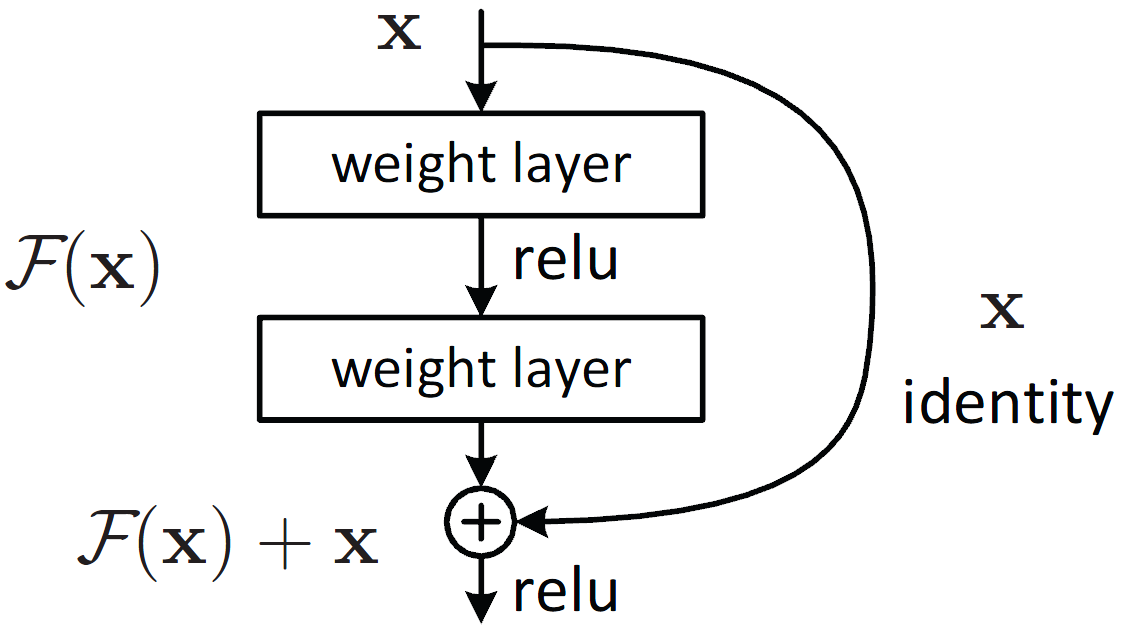
\includegraphics[width=0.95\linewidth]{figs/resnet_1.png}
\end{figure}
\end{minipage}
\begin{figure}
    \centering
    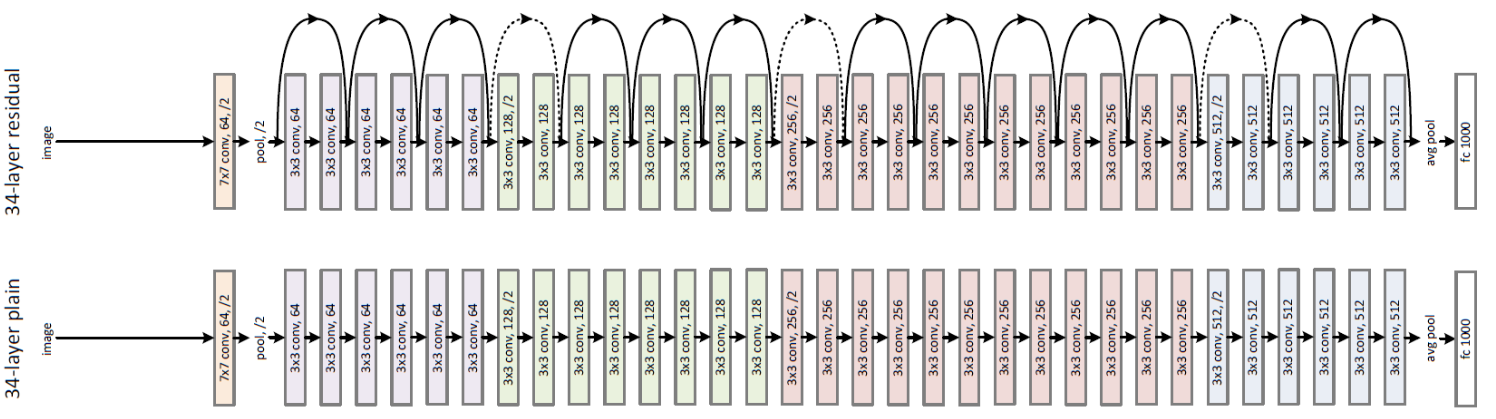
\includegraphics[width=\linewidth]{figs/resnet_2.png}
\end{figure}
\vfill
\hrule\medskip
{\scriptsize \href{https://arxiv.org/abs/1806.07366}{https://arxiv.org/abs/1806.07366}}   
\end{frame}
%=======
\begin{frame}{Neural ODE}
Consider ODE    
\vspace{-0.2cm}
\[
    \frac{d \bz(t)}{dt} = f(\bz(t), \btheta); \quad \bz(t_0) = \bz_0.
\]
\vspace{-0.2cm}
\begin{block}{Euler update step}
\vspace{-0.2cm}
\[
    \bz(t + \Delta t) = \bz(t) + \Delta t f(\bz(t), \btheta).
\]
\vspace{-0.2cm}
\end{block}
\begin{block}{Residual block}
\vspace{-0.2cm}
\[
    \bz_{t+1} = \bz_t + f(\bz_t, \btheta).
\]
\vspace{-0.2cm}
\end{block}
It is exactly Euler update step for solving ODE with $\Delta t = 1$! \\
Euler update step is unstable and trivial. \\
 \vfill
\hrule\medskip
{\scriptsize \href{https://arxiv.org/abs/1806.07366}{https://arxiv.org/abs/1806.07366}}   
\end{frame}
%=======
\begin{frame}{Neural ODE}
\begin{block}{Residual block}
\vspace{-0.2cm}
\[
    \bz_{t+1} = \bz_t + f(\bz_t, \btheta).
\]
\vspace{-0.2cm}
\end{block}
What happens as we add more layers and take smaller steps? \\
In the limit, we parameterize the continuous dynamics of hidden units using an ODE specified by a neural network: 
\[
    \frac{d \bz(t)}{dt} = f(\bz(t), t, \btheta); \quad \bz(t_0) = \bx; \quad \bz(t_1) = \by.
\]
\vspace{-0.2cm}
\begin{block}{Loss function}
\vspace{-0.2cm}
\begin{align*}
    L(\by) = L(\bz(t_1)) &= L\left( \bz(t_0) + \int_{t_0}^{t_1} f(\bz(t), t, \btheta) dt \right) \\ &= L\left(\text{ODESolve}(\bz(t_0), f, t_0,t_1, \btheta) \right)
\end{align*}
\vspace{-0.2cm}
\end{block}
 \vfill
\hrule\medskip
{\scriptsize \href{https://arxiv.org/abs/1806.07366}{https://arxiv.org/abs/1806.07366}}   
\end{frame}
%=======
\begin{frame}{Neural ODE}

\vspace{-0.2cm}
\begin{block}{Benefits}
\begin{itemize}
    \item memory efficient;
    \item adaptive computation;
    \item parameter efficient;
    \item scalable and invertible normalizing flows.
\end{itemize}
\end{block}
\begin{figure}
    \centering
    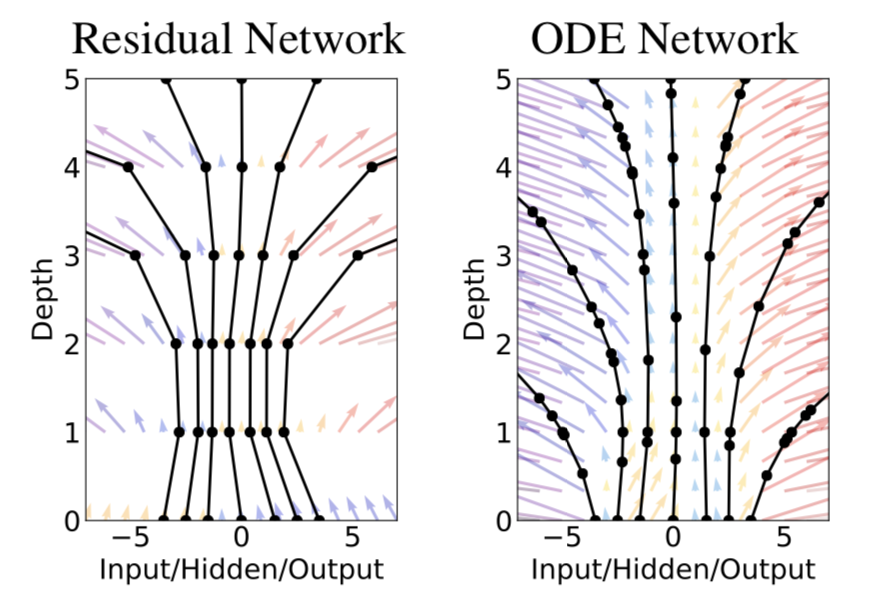
\includegraphics[width=0.55\linewidth]{figs/resnet_vs_neural_ode.png}
\end{figure}
 \vfill
\hrule\medskip
{\scriptsize \href{https://arxiv.org/abs/1806.07366}{https://arxiv.org/abs/1806.07366}}   
\end{frame}
%=======
\begin{frame}{Neural ODE}
\begin{block}{Loss function}
\vspace{-0.2cm}
\[
    L(\by) = L(\bz(t_1)) = L\left(\text{ODESolve}(\bz(t_0), f, t_0,t_1, \btheta) \right)
\]
\vspace{-0.2cm}
\end{block}
How to train such model? How to fit $\btheta$? How to compute efficiently $\frac{\partial L}{\partial \btheta}$? -- Pontryagin theorem!
\begin{block}{Adjoint function}
\vspace{-0.2cm}
\[
    \ba(t) = \frac{\partial L(\bz(t))}{\partial \bz(t)}
\]
\vspace{-0.2cm}
\end{block}
\begin{block}{Theorem}
\vspace{-0.2cm}
\[
    \frac{d \ba(t)}{dt} = - \ba(t)^T \frac{\partial f(\bz(t), t, \btheta)}{\partial \bz(t)}
\]
\end{block}
 \vfill
\hrule\medskip
{\scriptsize \href{https://arxiv.org/abs/1806.07366}{https://arxiv.org/abs/1806.07366}}   
\end{frame}
%=======
\begin{frame}{Neural ODE}
\begin{block}{Theorem}
\vspace{-0.2cm}
\[
    \frac{d \ba(t)}{dt} = - \ba(t)^T \frac{\partial f(\bz(t), t, \btheta)}{\partial \bz(t)}; \quad \ba(t) = \frac{\partial L(\bz(t))}{\partial \bz(t)}
\]
\end{block}

To obtain $\ba(t)$ along the trajectory we could solve this ODE backward in time, starting from the initial value $\ba(t_1) = \frac{\partial L(\bz(t_1))}{\partial \bz(t_1)}$.
\begin{block}{Theorem}
\vspace{-0.2cm}
\[
    \frac{dL}{d \btheta} = - \int_{t_0}^{t_1} \ba(t)^T \frac{\partial f(\bz(t), t, \btheta)}{\partial \btheta} dt.
\]
\end{block}
All these gradients could be computed at once.
\vfill
\hrule\medskip
{\scriptsize \href{https://arxiv.org/abs/1806.07366}{https://arxiv.org/abs/1806.07366}} 
\end{frame}
%=======
\begin{frame}{Continuous NF}
\begin{block}{Discrete NF}
\vspace{-0.2cm}
    \[
    \bz_{t+1} = f(\bz_t, \btheta); \quad \log p(\bz_{t+1}) = \log p(\bz_{t}) - \log \left| \det \frac{\partial f(\bz_t, \btheta)}{\partial \bz_{t}} \right| .
    \]
\vspace{-0.2cm}
Function $f$ should be bijective!
\end{block}
\begin{block}{Theorem}
\[
    \frac{\partial \log p(\bz(t))}{\partial t} = - \text{trace} \left( \frac{\partial f}{\partial \bz(t)} \right).
\]
Function $f$ is not necessary bijective! (uniformly Lipschitz continuous in $\bz$ and continuous in $t$).
\end{block}
\vfill
\hrule\medskip
{\scriptsize \href{https://arxiv.org/abs/1806.07366}{https://arxiv.org/abs/1806.07366}} 
\end{frame}
%=======
\begin{frame}{Continuous NF}
\[
    \log p(\bz(t_1)) = \log p(\bz(t_0)) - \int_{t_0}^{t_1} \text{trace} \left( \frac{\partial f}{\partial \bz} \right) dt.
\]
\begin{figure}
    \centering
    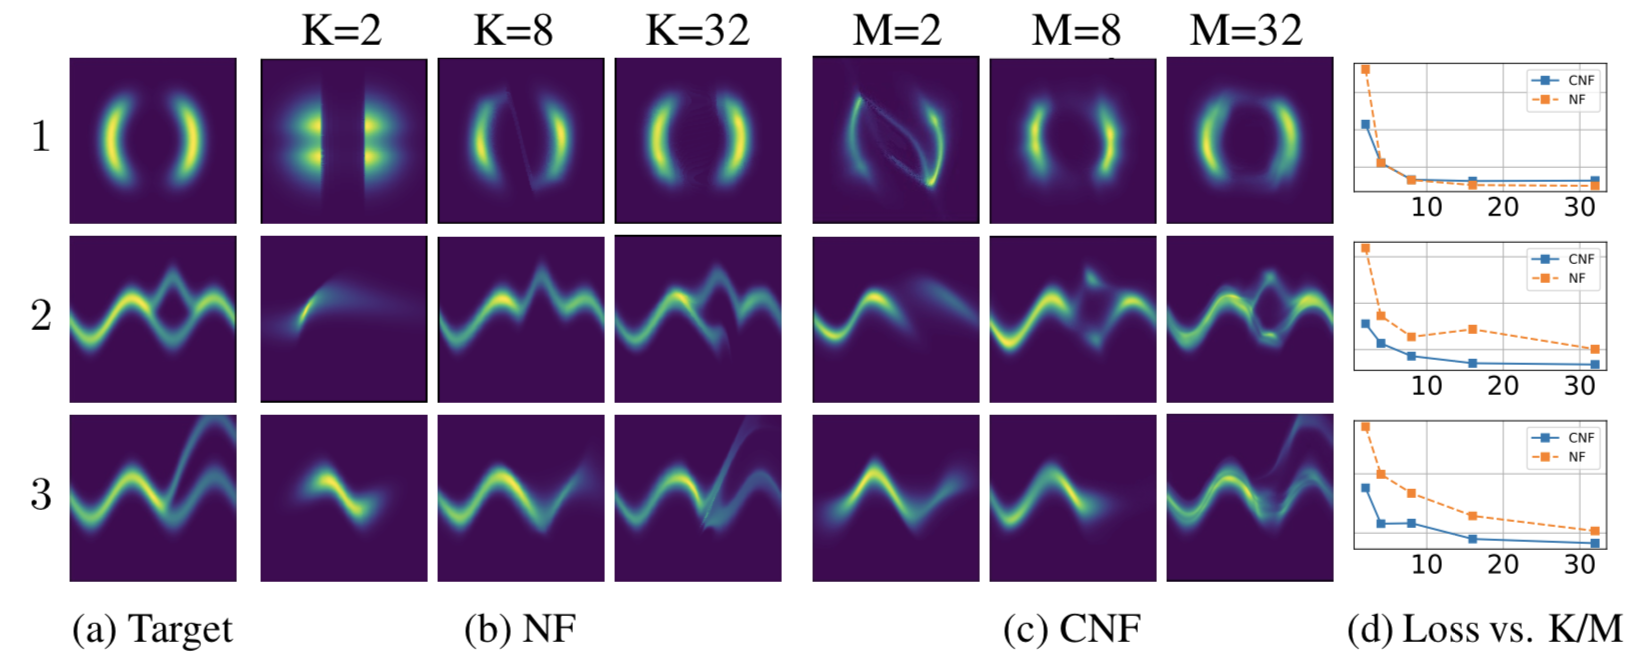
\includegraphics[width=0.5\linewidth]{figs/cnf.png}
\end{figure}
\vfill
\hrule\medskip
{\scriptsize \href{https://arxiv.org/abs/1806.07366}{https://arxiv.org/abs/1806.07366}} 
\end{frame}
%=======
\begin{frame}{FFJORD}
\begin{figure}
    \centering
    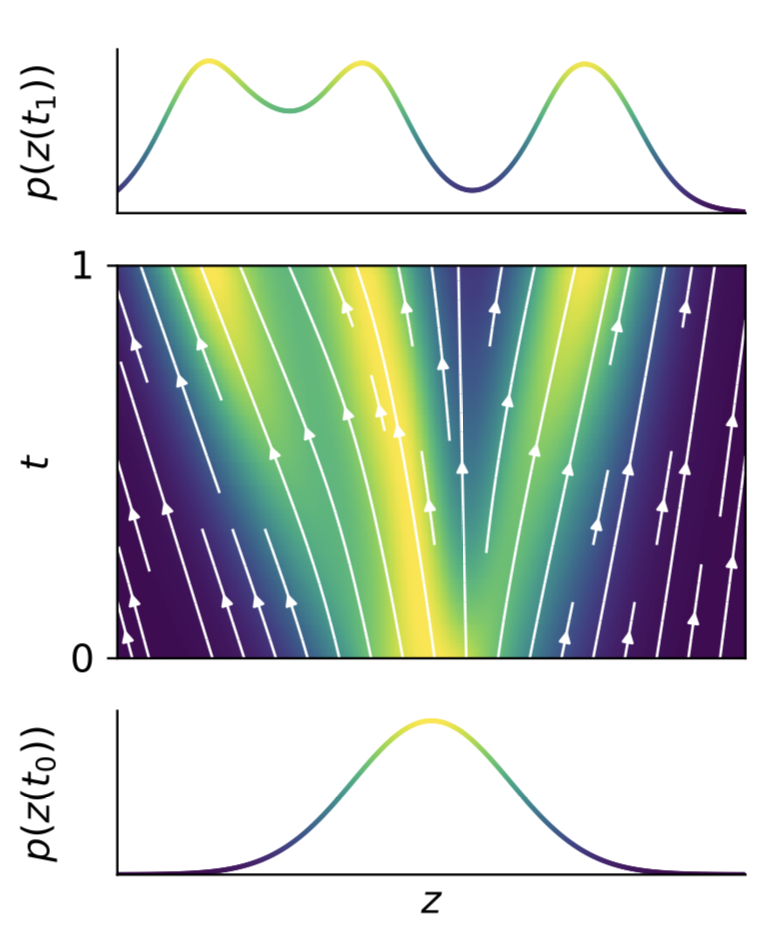
\includegraphics[width=0.5\linewidth]{figs/cnf_flow.png}
\end{figure}
\vfill
\hrule\medskip
{\scriptsize \href{https://arxiv.org/abs/1810.01367}{https://arxiv.org/abs/1810.01367}} 
\end{frame}
%=======
\begin{frame}{FFJORD}
\begin{block}{Hutchinson's trace estimator}
\[
    \text{trace}(A) = \mathbb{E}_{p(\bepsilon)} \left[ \bepsilon^T A \bepsilon \right]; \quad \mathbb{E} [\bepsilon] = 0; \quad \text{Cov} (\bepsilon) = I.
\]
\end{block}
\begin{align*}
    \log p(\bz(t_1)) &= \log p(\bz(t_0)) - \int_{t_0}^{t_1} \text{trace} \left( \frac{\partial f}{\partial \bz} \right) dt \\
    &= \log p(\bz(t_0)) - \int_{t_0}^{t_1} \mathbb{E}_{p(\bepsilon)} \left[ \bepsilon^T \frac{\partial f}{\partial \bz} \bepsilon \right] dt \\
    &= \log p(\bz(t_0)) - \mathbb{E}_{p(\bepsilon)} \int_{t_0}^{t_1} \left[ \bepsilon^T \frac{\partial f}{\partial \bz} \bepsilon \right] dt.
\end{align*}
This reduces the cost from quadratic to linear.\\
\vfill
\hrule\medskip
{\scriptsize \href{https://arxiv.org/abs/1810.01367}{https://arxiv.org/abs/1810.01367}} 
\end{frame}
%=======
\begin{frame}{FFJORD}
\begin{figure}
    \centering
    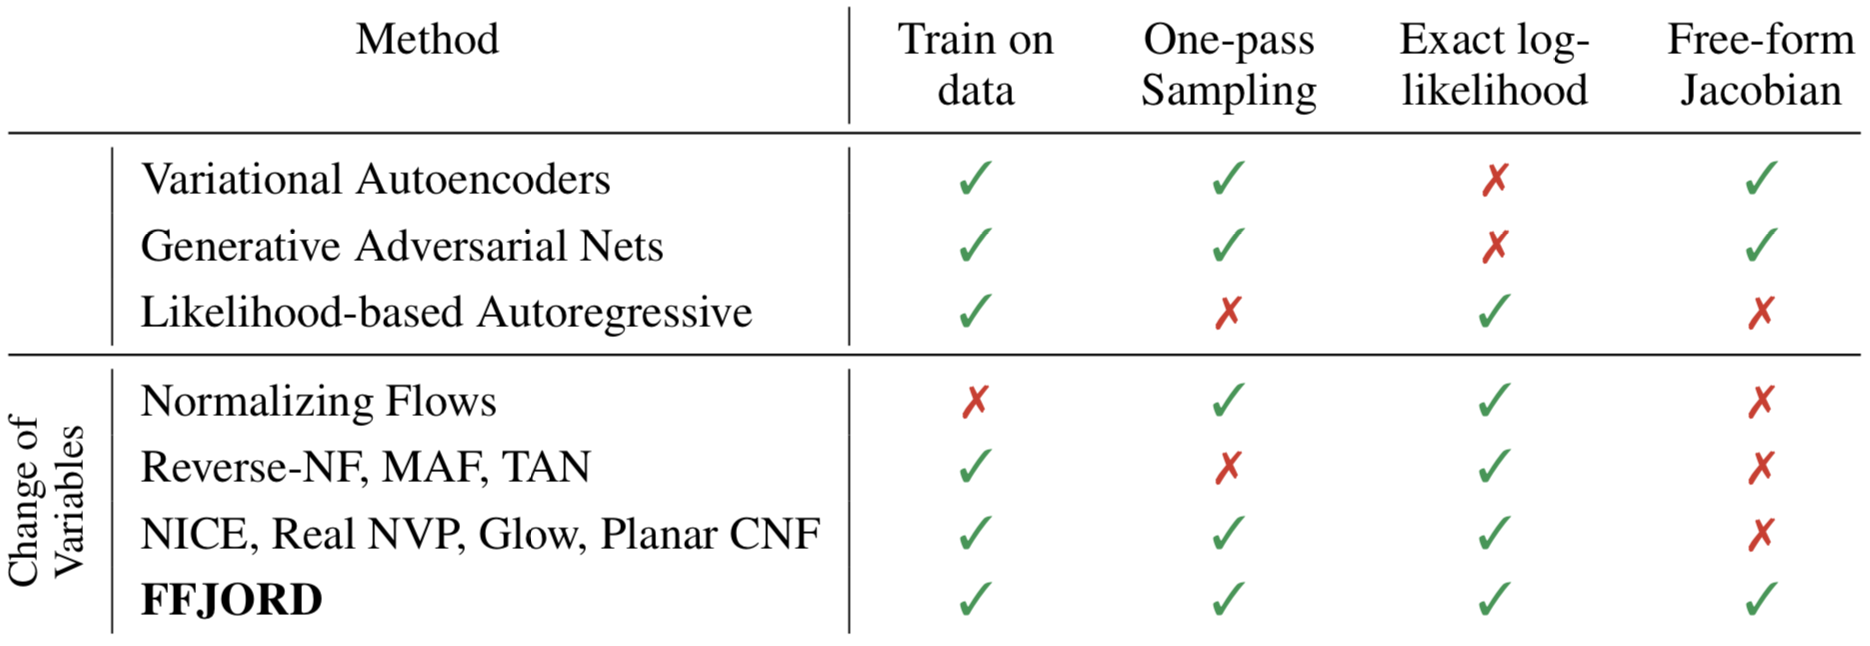
\includegraphics[width=\linewidth]{figs/flow_comparison.png}
\end{figure}
\vfill
\hrule\medskip
{\scriptsize \href{https://arxiv.org/abs/1810.01367}{https://arxiv.org/abs/1810.01367}} 
\end{frame}
%=======
\begin{frame}{FFJORD}
\begin{figure}
    \centering
    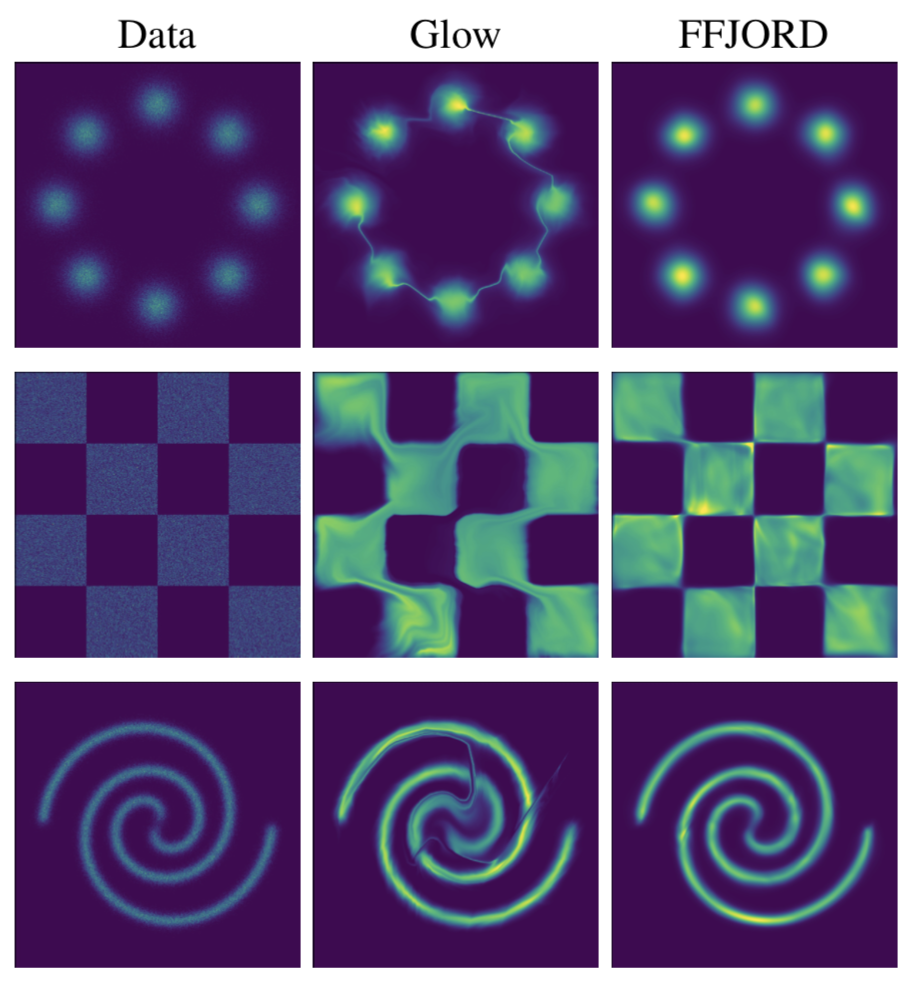
\includegraphics[width=0.6\linewidth]{figs/ffjord.png}
\end{figure}
\vfill
\hrule\medskip
{\scriptsize \href{https://arxiv.org/abs/1810.01367}{https://arxiv.org/abs/1810.01367}} 
\end{frame}
%=======
\begin{frame}{Discrete VAE}
	\begin{itemize}
		\item Before we have discussed VAE with \textbf{continuous} latent variables.
		\item VAE suffers from posterior collapse if the decoder too powerful (PixelVAE, VLAE tries to solve this problem).
		\item \textbf{Discrete} representations are potentially a more natural fit for many of the modalities.
		\item Powerful autoregressive models (like PixelCNNN) have been developed for modelling distributions over discrete variables.
		\item However, to construct the model with discrete representations is not so easy (e.g. variance of such estimators is a problem).
	\end{itemize}
	\vfill
	\hrule\medskip
	{\scriptsize \href{https://arxiv.org/abs/1711.00937}{https://arxiv.org/abs/1711.00937}} 
\end{frame}
%=======
\begin{frame}{Vector Quantized VAE}
	\begin{itemize}
		\item Latent embedding space $\{\be_j\}_{j=1}^K$, where $\be_j \in \bbR_D$, $K$ is the size of the discrete latent space.
		\item $\bz_e(\bx)$ is the encoder output.
		\item $z$ is the discrete random variable calculated by a nearest neighbour look-up using the shared embedding space. The posterior categorical distribution is defined as 
		\[
			q(z = k | \bx) = \begin{cases}
				1 , \quad \text{for } k = \argmin_j \| \bz_e(\bx) - \be_j \| \\
				0, \quad \text{otherwise}.
			\end{cases}
		\]
		
		\item VAE proposal distribution $q(z | \bx)$ is deterministic. If prior $p(z)$ is a uniform then $KL(q(z| \bx) || p(z))$ term in ELBO is constant (equals to $\log K$).
		\item Quantized representation is defined as follows
		\[
			\bz_q(\bx) = \be_k, \quad \text{where } k = \argmin_j \| \bz_e(\bx) - \be_j \| 
		\] 
		
	\end{itemize}
	\vfill
	\hrule\medskip
	{\scriptsize \href{https://arxiv.org/abs/1711.00937}{https://arxiv.org/abs/1711.00937}} 
\end{frame}
%=======
\begin{frame}{Vector Quantized VAE}
	\begin{figure}
		\centering
		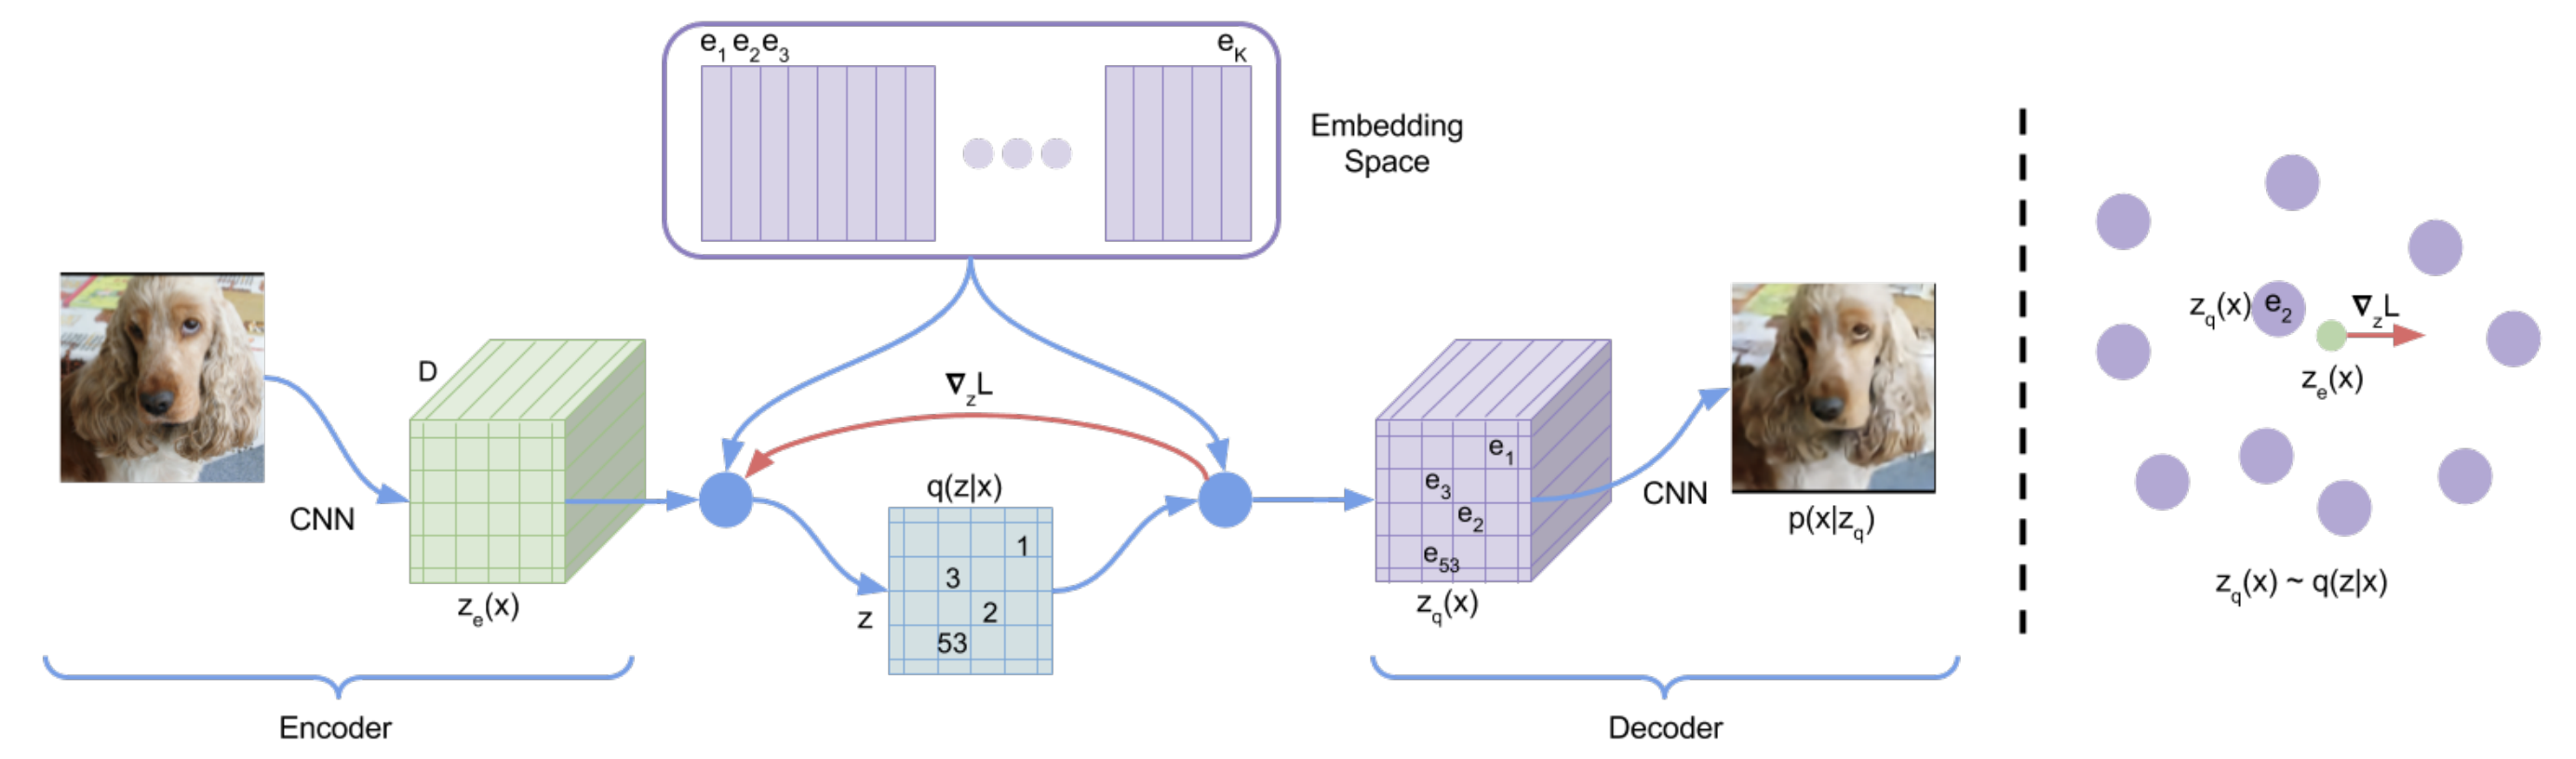
\includegraphics[width=\linewidth]{figs/vqvae}
	\end{figure}
	\begin{block}{Objective}
		\vspace{-0.3cm}
		\[
			\log p(\bx | \bz_q(\bx)) + \| \text{sg} (\bz_e(\bx)) - \bz_q(\bx) \| + \beta \| \bz_e(\bx) - \text{sg}(\bz_q(\bx)) \|
		\]
	\end{block}
	\begin{itemize}
		\item Quantization operation is not differentiable.
		\item Straight-through gradient estimation is used to backpropagate the quantization operation.
	\end{itemize}
	\vfill
	\hrule\medskip
	{\scriptsize \href{https://arxiv.org/abs/1711.00937}{https://arxiv.org/abs/1711.00937}} 
\end{frame}
%=======
\begin{frame}{Vector Quantized VAE}
	\begin{figure}
		\centering
		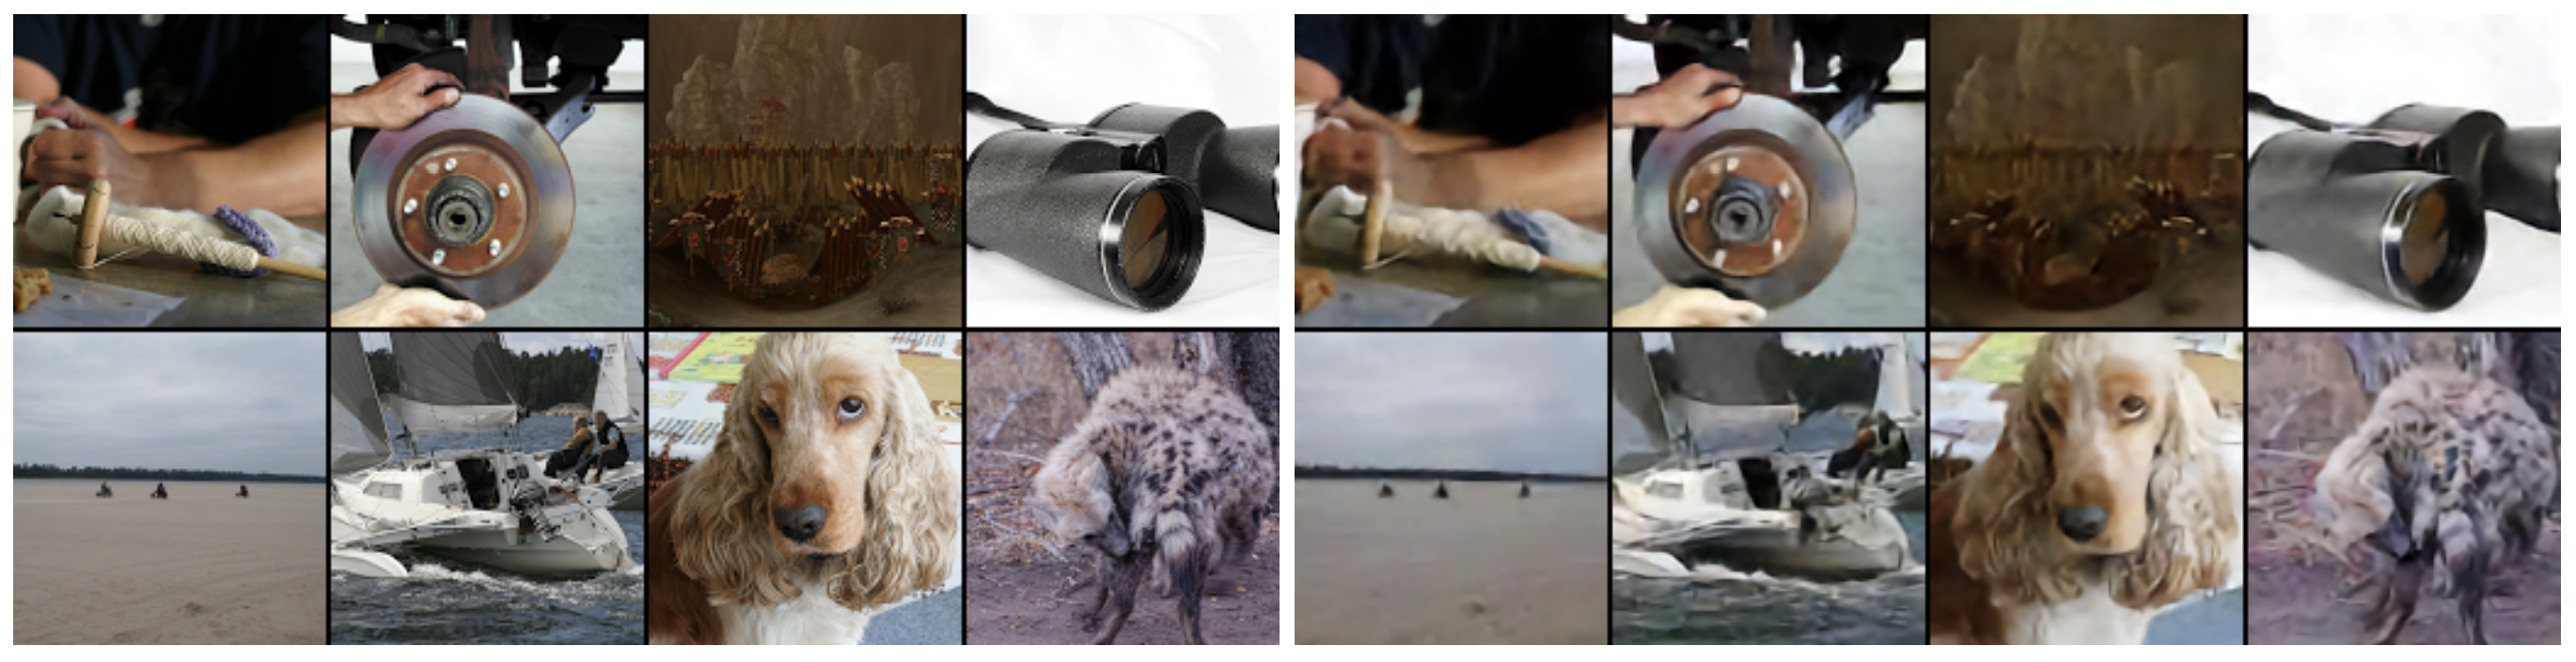
\includegraphics[width=\linewidth]{figs/vqvae_results}
	\end{figure}
	\vfill
	\hrule\medskip
	{\scriptsize \href{https://arxiv.org/abs/1711.00937}{https://arxiv.org/abs/1711.00937}} 
\end{frame}
%=======
\begin{frame}{References}
{\tiny
\begin{itemize}
    \item Neural Ordinary Differential Equations \\
    \href{https://arxiv.org/abs/1806.07366}{https://arxiv.org/abs/1806.07366} \\
    \textbf{Summary:} New interpretation of resnets as special case of ode. 
    Discrete sequence of layers  are replaced with continuous dynamic. ODESolver is used for backpropagation. Pontryagin theorem gives the analog of the chain rule. Continuous version \\ of normalizing flow is constructed.
    
    \item \textbf{FFJORD:} Free-form Continuous Dynamics for Scalable Reversible Generative Models \\
    \href{https://arxiv.org/abs/1810.01367}{https://arxiv.org/abs/1810.01367} \\
    \textbf{Summary:} Continuous version of NF is investigated. 
    Jacobian computation cost is reduced to O(D) by using Hutchinson’s \\ trace estimator. 
    
    \item \textbf{VQ-VAE:} Neural discrete representation learning \\
    \href{https://arxiv.org/abs/1711.00937}{https://arxiv.org/abs/1711.00937} \\
    \textbf{Summary:} Discrete latent representation for VAE. Nearest neighbor lookup table quantization is used. Learned powerful PixelCNN prior in the latent space.
\end{itemize}
}
\end{frame}
\end{document} 